\section{Industrial Deployments and Human Factors}\label{sec:deployment}

Production reports share one caveat: every firm defines ``success'' differently, so the headline numbers in Fig.~\ref{fig:field} measure different things and must not be ranked against each other.

\textbf{Industrial deployments.}
Google's AutoCommenter reports a comment-resolution rate of about 40\%, and 80\% of raw comments would have landed on unmodified lines before filtering. A large A/B test with about half of Google's developers showed no significant change in review duration~\cite{vijayvergiya2024ai}.
ByteDance's BitsAI-CR reports an Outdated Rate (share of flagged lines later modified) of 26.7\% for Go against 35--46\% for human comments; second-week retention was 61.64\%~\cite{sun2025bitsai}.
At Atlassian, RovoDev's code-resolution rate was 38.70\% against 44.45\% for human comments, and median PR cycle time fell 30.8\% (observational, not randomised)~\cite{tantithamthavorn2026rovodev}.
Meta's fine-tuned model reached a 19.7\% ActionableToApplied rate, the share of suggested patches that authors apply~\cite{maddila2025ai}.
At Beko, 73.8\% of PR-Agent comments were marked ``Resolved'', but resolution is a mandatory label set before merge, and average PR closure time rose from 5h52m to 8h20m~\cite{cihan2025automated}. A follow-up found that LLM-judge agreement with engineers' labels was only 0.44--0.62~\cite{karakaya2026understanding}.
At Mozilla and Ubisoft, reviewers accepted 8.1\% and 7.2\% of RevMate's comments~\cite{olewicki2024impact}.
Ericsson has reported only an experience report and an offline validation of a multi-agent reviewer (96\% of more than 200 flagged issues validated), not field acceptance rates~\cite{ramesh2025automated}.

\begin{figure}[t]
\centering
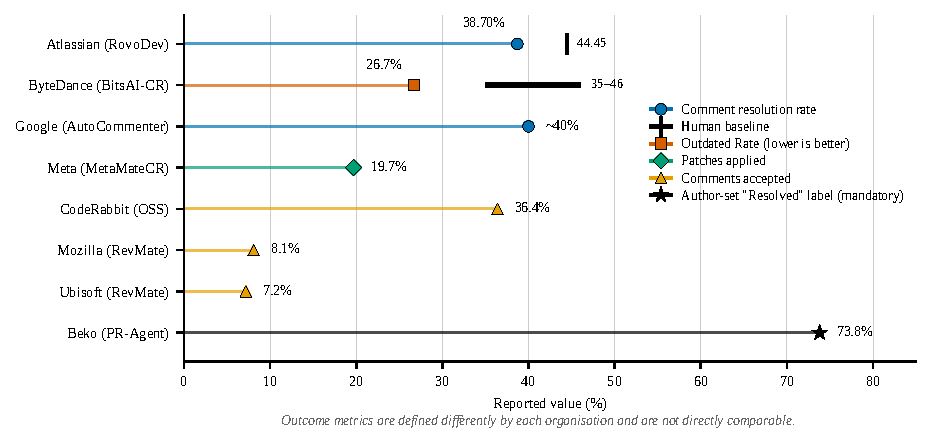
\includegraphics[width=\linewidth]{figures/field_outcomes.pdf}
\caption{Field outcomes by organisation, with the human baseline where one was measured. Markers differ by metric type; the values are not comparable across studies.}
\label{fig:field}
\end{figure}

\textbf{Open-source mining.}
In 31,073 CodeRabbit review/feedback pairs, 36.4\% were accepted and 56.3\% rejected, mainly as false positives and redundancy~\cite{lin2026agentic}.

\textbf{Controlled evidence.}
In the one controlled experiment (29 experts), reviewers given an LLM review concentrated on the flagged locations and found more low-severity but not more high-severity issues, with no time saved: an anchoring effect~\cite{tufano2025deep}.
The evidence on cycle time conflicts: Atlassian observed a reduction, Beko an increase, and Google no significant change.
The only randomised trial, at Meta, found that showing AI patches to reviewers slowed reviews by more than 5\%, while showing them only to authors removed the regression~\cite{maddila2025ai}.

\textbf{Human and organisational factors.}
Interviewees reported that cognitive load sometimes rises because of the LLM's excessive details~\cite{alami2025human}. Atlassian's 35.6\% drop in human comments per PR raises an open question: do workload savings come from displacing human scrutiny? Privacy is handled mainly by design: Google, Meta and ByteDance run in-house models, whereas Beko and Mozilla/Ubisoft used third-party APIs~\cite{sun2025bitsai,cihan2025automated,olewicki2024impact}.
